\documentclass[border=10pt]{standalone}
\usepackage{pgfplots}
\pgfplotsset{compat=1.18}
\begin{document}
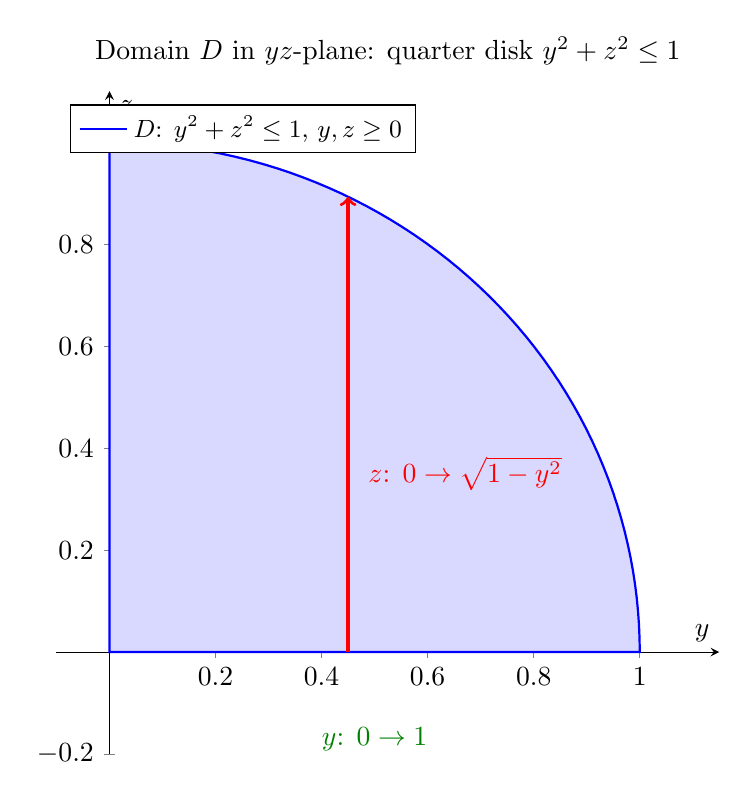
\begin{tikzpicture}
\begin{axis}[
    xlabel={$y$}, ylabel={$z$},
    xmin=-0.1, xmax=1.15, ymin=-0.2, ymax=1.1,
    axis lines=middle,
    width=10cm, height=10cm,
    title={Domain $D$ in $yz$-plane: quarter disk $y^2+z^2\le 1$},
    legend style={font=\small, at={(0.02,0.98)}, anchor=north west},
]
% Quarter disk
\addplot[domain=0:90, samples=60, variable=\t, fill=blue!15, draw=blue, thick]
    ({cos(\t)}, {sin(\t)}) \closedcycle;
\addlegendentry{$D$: $y^2+z^2\le 1$, $y,z\ge 0$}
% z-slice arrow at y=0.45
\draw[->, red, very thick] (axis cs:0.45,0) -- (axis cs:0.45,{sqrt(1-0.45^2)});
\node[red, anchor=west] at (axis cs:0.47,0.35) {$z$: $0\to\sqrt{1-y^2}$};
\node[green!50!black, anchor=north] at (axis cs:0.5,-0.13) {$y$: $0\to 1$};
\end{axis}
\end{tikzpicture}
\end{document}